%!TEX root = report.tex

\section{Methodology}

%Methodology/Algorithm: What method or algorithm are you proposing? If there are existing implementations, will you use them and how? How do you plan to improve or modify such implementations?

Our project will start from the method proposed by \cite{yang2017attention}, which is summarized in Figure \ref{Fig:Flow} (black lines). The model consider the author information and sentence information separately: each node (author) in the network is assigned an embedding vector using the LINE algorithm (\cite{tang2015line}), and then is (softly) assigned each cluster on the network based on the embedding. Each cluster has its own model, which is a CNN model combined with max pool layer. This model provides a baseline in our project.

\begin{figure}[htbp] %  figure placement: here, top, bottom, or page
   \centering
   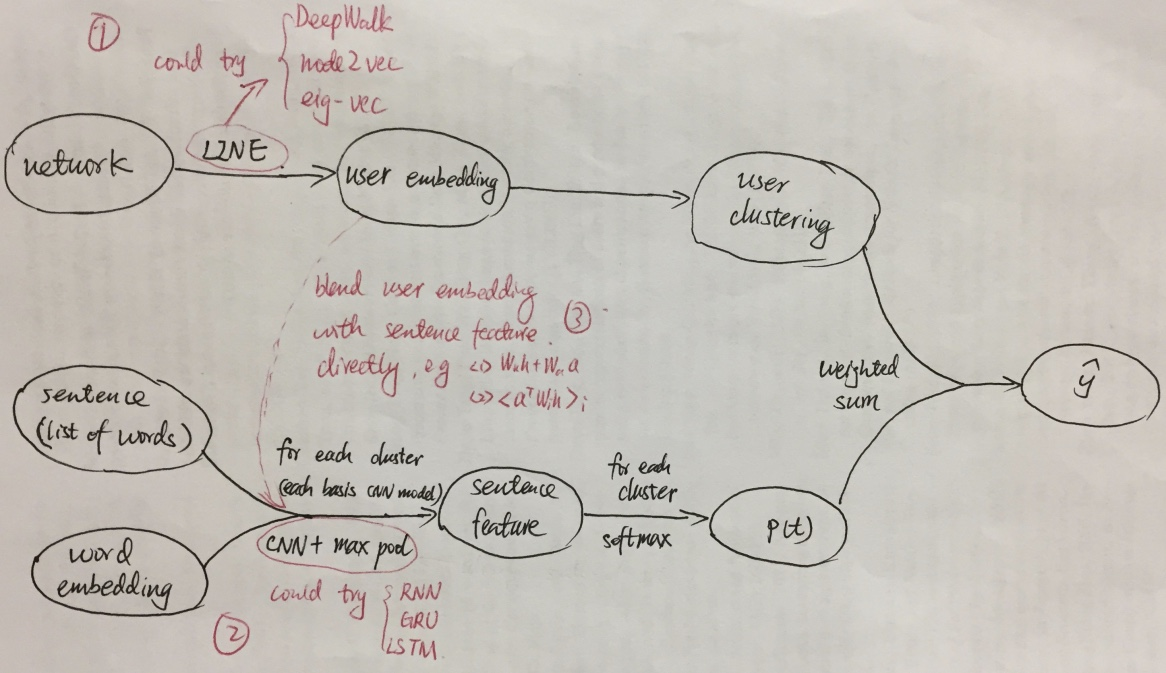
\includegraphics[width=5.2in]{flow.jpg} 
   \caption{General Methodology}
   \label{Fig:Flow}
\end{figure}



We are going to extend this model in three aspects, as is illustrated in the red lines in Figure \ref{Fig:Flow}. To be specific, 
\begin{enumerate}   [(1)]
%\setcounter{enumi}{3}
\item Using other node embedding methods in network analysis, such as \textit{DeepWalk} (\cite{perozzi2014deepwalk}) and \textit{node2vec} (\cite{grover2016node2vec});
\item Explore other methods to combine author information and sentence information, especially the bilinear form $a^T W h$ which measures the interaction between author and sentence. Here $a$ is the author embedding and $h$ is the sentence embedding.
\item Explore other models in sentiment analysis, such as RNN, GRU, and LSTM.
\end{enumerate}
